% !TeX spellcheck = cs_CZ
%=========================== Kapitola: Mody =======================================================
\setchaptertoc
\chapter{Mody}\label{fyz:IchapIL}

  \section{Odraz vln}\label{fyz:IchapILsecI}
  \section{Vlny v ohraničené oblasti, vlastní frekvence}\label{fyz:IchapILsecII}
  \section{Dvojrozměrné mody}\label{fyz:IchapILsecIII}
  \section{Vázaná kyvadla}\label{fyz:IchapILsecIV}
  \section{Lineární soustavy}\label{fyz:IchapILsecV}
  \section{Příklady a cvičení}\label{fyz:IchapILsecVI}

    \begin{figure}[ht!] %\ref{fyz:fig0446}
      \centering
      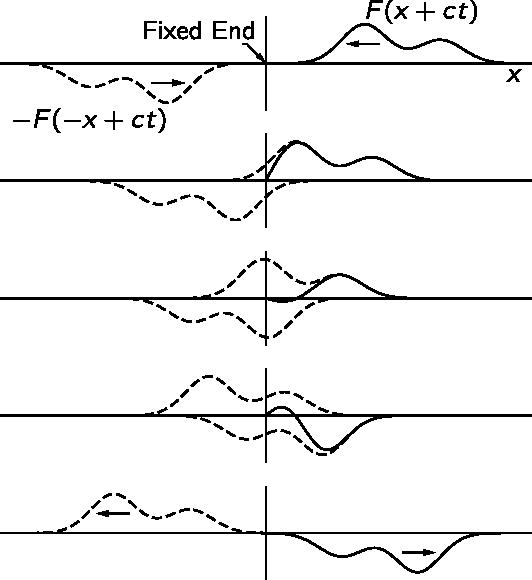
\includegraphics[width=0.7\linewidth]{fyz_fig0446.pdf}
      \caption{ 
               (\cite[s.~707]{Feynman01})}
      \label{fyz:fig0446}
    \end{figure}

    \begin{figure}[ht!] %\ref{fyz:fig0447}
      \centering
      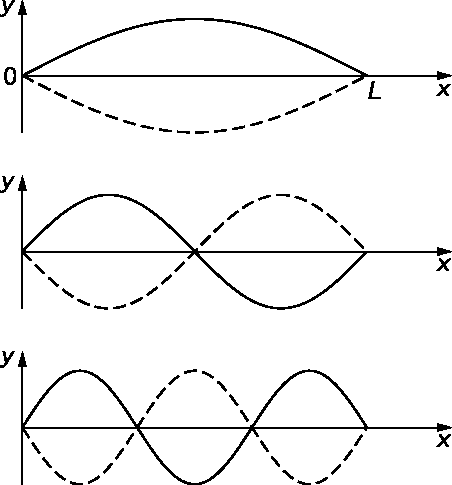
\includegraphics[width=0.7\linewidth]{fyz_fig0447.pdf}
      \caption{ 
               (\cite[s.~707]{Feynman01})}
      \label{fyz:fig0447}
    \end{figure}

    \begin{figure}[ht!] %\ref{fyz:fig0448}
      \centering
      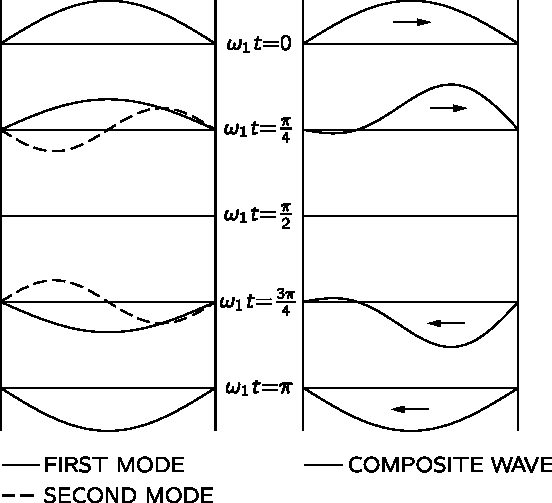
\includegraphics[width=0.7\linewidth]{fyz_fig0448.pdf}
      \caption{ 
               (\cite[s.~707]{Feynman01})}
      \label{fyz:fig0448}
    \end{figure}

    \begin{figure}[ht!] %\ref{fyz:fig0449}
      \centering
      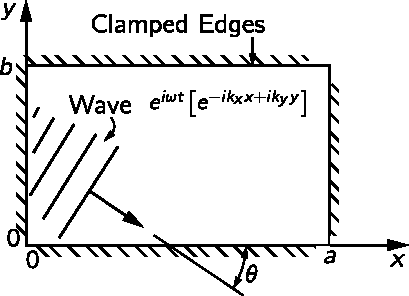
\includegraphics[width=0.7\linewidth]{fyz_fig0449.pdf}
      \caption{ 
               (\cite[s.~707]{Feynman01})}
      \label{fyz:fig0449}
    \end{figure}

    \begin{figure}[ht!] %\ref{fyz:fig0450}
      \centering
      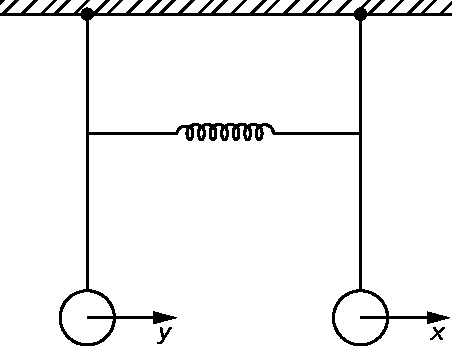
\includegraphics[width=0.7\linewidth]{fyz_fig0450.pdf}
      \caption{ 
               (\cite[s.~707]{Feynman01})}
      \label{fyz:fig0450}
    \end{figure}
    9\todo[inline]{Kapitola fey1ch49 je zcela prázdná, pouze obrázky} 
%---------------------------------------------------------------------------------------------------